\section{Network Applications and Socket Programming}
\subsection{Network Applications}
\begin{figure}[H]
    \tikzsetnextfilename{client-server-v-p2p}
    \begin{tikzpicture}
        \node[white, draw=blue, rectangle, minimum width=2cm, minimum height=1cm, top color=blue!30!white, bottom color=blue!60!white] (s) {Server};
        \node[below left=1cm and -0.5cm of s,white, draw=blue, rectangle, minimum width=2cm, minimum height=1cm, top color=blue!30!white, bottom color=blue!60!white] (c1) {Client};
        \node[below right=1cm and -0.5cm of s,white, draw=blue, rectangle, minimum width=2cm, minimum height=1cm, top color=blue!30!white, bottom color=blue!60!white] (c2) {Client};

        \node[right=3cm of s,white, draw=blue, rectangle, minimum width=2cm, minimum height=1cm, top color=blue!30!white, bottom color=blue!60!white] (n1) {Node};
        \node[right=of n1,white, draw=blue, rectangle, minimum width=2cm, minimum height=1cm, top color=blue!30!white, bottom color=blue!60!white] (n2) {Node};
        \draw[<->,blue!60!white] (s) -- (c1);
        \draw[<->,blue!60!white] (s) -- (c2);
        \draw[<->,blue!60!white] (n1) -- (n2);
        \path ([yshift=-0.5cm]c1.south) -- ([yshift=-0.5cm]c2.south) node[pos=0.5] () {Client-Server};
        \path ([yshift=-0.5cm]n1.south) -- ([yshift=-0.5cm]n2.south) node[pos=0.5] () {Peer-to-Peer};

        \node[below right =0.5cm and 1cm of c2] () {Hybrid};
    \end{tikzpicture}
\end{figure}
\url{https://en.wikipedia.org/wiki/Peer-to-peer}
\subsection{Inter-Application Communication}
\begin{multicols}{2}
    \begin{itemize}[nosep]
        \item Need a way to send and receive messages
        \item Inter-process communication
        \item Need naming, routing, transport
        \item Transport using TCP and UDP
              \begin{itemize}[nosep]
                  \item On top of IP
              \end{itemize}
    \end{itemize}
    \begin{figure}[H]
        \tikzsetnextfilename{interapp-comm}
        \begin{tikzpicture}
            \node[white, draw=blue, rectangle, minimum width=2cm, minimum height=1cm, top color=blue!30!white, bottom color=blue!60!white] (s) {Server};
            \node[below =4cm of s,white, draw=blue, rectangle, minimum width=2cm, minimum height=1cm, top color=blue!30!white, bottom color=blue!60!white] (client) {Client};
            \draw[<->, blue!60!white] (s) -- (client);
            \node[below =1cm of s,white, draw=blue, cloud, minimum size=2cm, top color=blue!30!white, bottom color=blue!60!white] (cloud) {};
        \end{tikzpicture}
    \end{figure}
\end{multicols}
\subsection{Application Protocols}
\begin{itemize}[nosep]
    \item Messages between processes, typically encapsulated within TCP or UDP
    \item Need agreement between
          \begin{itemize}[nosep]
              \item Sending process
              \item Receiving process
          \end{itemize}
\end{itemize}
\subsection{Network Time Service}
\begin{figure}[H]
    \tikzsetnextfilename{network-time-service}
    \begin{tikzpicture}
        \node[rounded corners,white, draw=blue, rectangle, minimum width=2cm, minimum height=1cm, top color=blue!30!white, bottom color=blue!60!white] (l) {Laptop};
        \node[rounded corners,right=4cm of l, white, draw=blue, rectangle, minimum width=2cm, minimum height=1cm, top color=blue!30!white, bottom color=blue!60!white] (s) {Server};

        \draw[blue!60!white,->] ([yshift=0.2cm]l.north east) -- ([yshift=0.2cm]s.north west) node[pos=0.1,label=above:{1.}] () {};
        \draw[blue!60!white,->] ([yshift=-0.2cm]s.south west) -- ([yshift=-0.2cm]l.south east) node[pos=0.9,label=below:{1.}] () {};

        \node[below=of s,align=center] () {Atomic clock\\facility};

        \path ([yshift=1cm]l.north east) -- ([yshift=1cm]s.north west) node[pos=0.5,label=above:{Client-server or peer-to-peer?}] () {};
    \end{tikzpicture}
\end{figure}
\subsection{Protocol Timing Diagram}
\begin{figure}[H]
    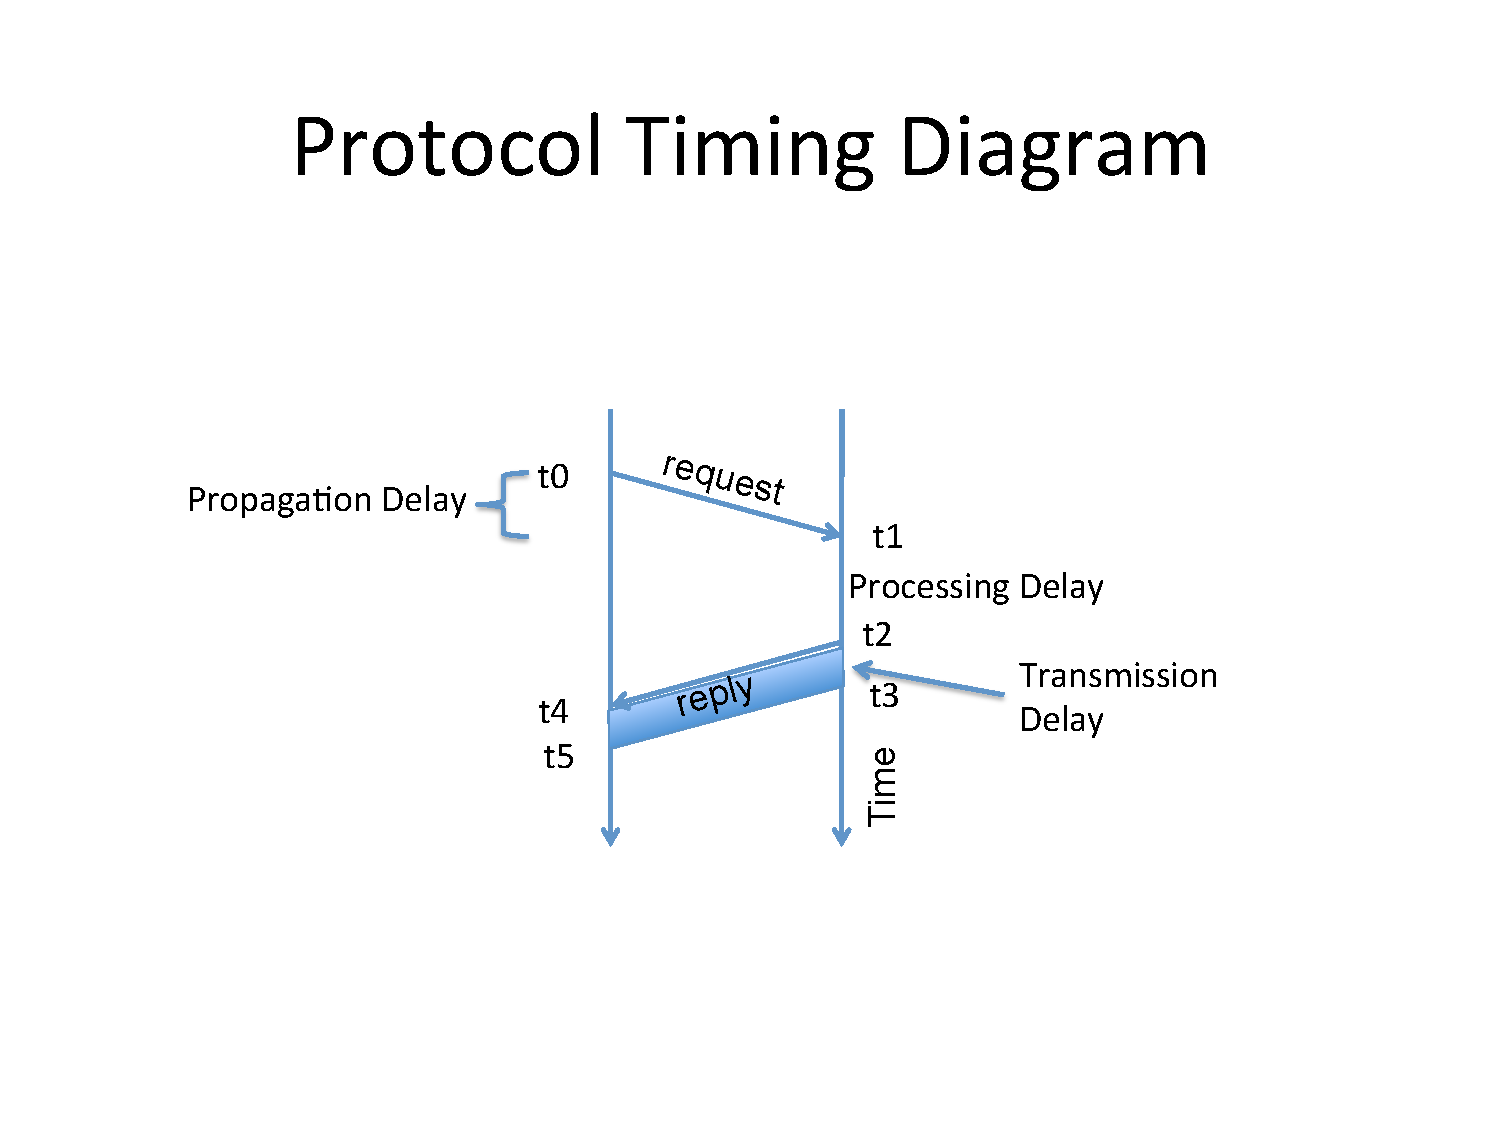
\includegraphics[width=\textwidth]{lazy/protocol.pdf}
\end{figure}
\subsection{Cloud-based File Backup Application}
\begin{itemize}[nosep]
    \item Client-server or peer-to-peer?
    \item Where do the applications run?
    \item Who/how to run these applications?
    \item What messages are exchanged?
\end{itemize}
\begin{figure}[H]
    \tikzsetnextfilename{cloud-backup}
    \begin{tikzpicture}
        \node[rounded corners,white, draw=blue, rectangle, minimum width=2cm, minimum height=1cm, top color=blue!30!white, bottom color=blue!60!white] (l) {Laptop};
        \node[rounded corners,right=4cm of l, white, draw=blue, rectangle, minimum width=2cm, minimum height=1cm, top color=blue!30!white, bottom color=blue!60!white] (s) {Server};

        \draw[blue!60!white,->] ([yshift=0.2cm]l.north east) -- ([yshift=0.2cm]s.north west);
        \draw[blue!60!white,->] ([yshift=-0.2cm]s.south west) -- ([yshift=-0.2cm]l.south east);

        \path ([yshift=0.2cm]l.north east) -- ([yshift=0.2cm]s.north west) node[pos=0.1,label=above:{3.}] () {};
        \path ([yshift=-0.2cm]s.south west) -- ([yshift=-0.2cm]l.south east) node[pos=0.9,label=below:{1.}] () {};
        \path ([yshift=0.5cm]l.north east) -- ([yshift=0.5cm]s.north west) node[pos=0.1,label=above:{2.}] () {};
        \path ([yshift=-0.5cm]s.south west) -- ([yshift=-0.5cm]l.south east) node[pos=0.9,label=below:{2.}] () {};
        \path ([yshift=0.8cm]l.north east) -- ([yshift=0.8cm]s.north west) node[pos=0.1,label=above:{1.}] () {};
        \path ([yshift=-0.8cm]s.south west) -- ([yshift=-0.8cm]l.south east) node[pos=0.9,label=below:{3.}] () {};
    \end{tikzpicture}
\end{figure}
\subsection{Socket Programming}
\subsection{Using TCP/IP}
\begin{itemize}[nosep]
    \item How can applications use the network?
    \item \emph{Sockets} API
          \begin{itemize}[nosep]
              \item Originall from BS, widely implemented (*BSD, Linux, Mac OS X, Windows, \dots)
              \item Higher-level APIs build on them
          \end{itemize}
    \item After basic setup, much like files
\end{itemize}
One could test network protocols with read/write on a file
\begin{figure}[H]
    \tikzsetnextfilename{socket-file}
    \begin{tikzpicture}
        \node[white, draw=blue, rectangle, minimum width=2cm, minimum height=1cm, top color=blue!30!white, bottom color=blue!60!white] (f) {File};
        \node[rounded corners,above left=1cm and -0.5cm of f,white, draw=blue, rectangle, minimum width=2cm, minimum height=1cm, top color=blue!30!white, bottom color=blue!60!white] (c) {Client};
        \node[rounded corners,above right=1cm and -0.5cm of f,white, draw=blue, rectangle, minimum width=2cm, minimum height=1cm, top color=blue!30!white, bottom color=blue!60!white] (s) {Server};

        \draw[blue!60!white, <->] (c) -- (f);
        \draw[blue!60!white, <->] (s) -- (f);
    \end{tikzpicture}
\end{figure}
\subsection{System Calls}
\begin{itemize}[nosep]
    \item Problem: how to access resources other than the CPU
          \begin{itemize}[nosep]
              \item Disk, netowrk, terminal, other processes
              \item CPU prohibits instructions that would access devices
              \item Only privileged OS kernel can access devices
          \end{itemize}
    \item Kernel supplies well-defined system call interface
          \begin{itemize}[nosep]
              \item Applications request I/O oeprations through syscalls
              \item Set up syscall arguments and trap to kernel
              \item Kernel performs operation and returns result
          \end{itemize}
    \item Higher-level functions built on syscall interface
          \begin{itemize}[nosep]
              \item \mintinline{c}|printf|, \mintinline{c}|scanf|, \mintinline{c}|gets|, all user-level code
          \end{itemize}
\end{itemize}
\subsection{File Descriptors}
\begin{itemize}[nosep]
    \item Most I/O in Unix done through \emph{file descriptors}
          \begin{itemize}[nosep]
              \item Integer \emph{handles} to per-process table in kernel
          \end{itemize}
    \item \mintinline{c}|int open(char *path, int flags, ...);|
    \item Returns file descriptor, used for all I/O to file
\end{itemize}
\url{https://en.wikipedia.org/wiki/File_descriptor}
\subsection{Error Returns}
\begin{itemize}[nosep]
    \item What if \mintinline{c}|open| fails? Return \mintinline{c}|-1| (invalid file descriptor)
    \item Most system calls return \mintinline{c}|-1| on failure
          \begin{itemize}[nosep]
              \item Specific type of error in gobal \mintinline{c}|int errno|
          \end{itemize}
    \item \mintinline{c}|#include <sys/errno.h>| for possible values
          \begin{itemize}[nosep]
              \item \mintinline{c}|2| = \mintinline{c}|ENOENT| ``no such file or directory''
              \item \mintinline{c}|13| = \mintinline{c}|EACCES| ``permission denied''
          \end{itemize}
\end{itemize}
\subsection{Some operations on File Descriptors}
\begin{itemize}[nosep]
    \item \mintinline{c}|ssize_t read(int fd, void* buf, int nbytes);|
          \begin{itemize}[nosep]
              \item Returns number of bytes read
              \item Returns \mintinline{c}|0| bytes at end of file, or \mintinline{c}|-1| on error
          \end{itemize}
    \item \mintinline{c}|ssize_t write(int fd, void* buf, int nbytes);|
          \begin{itemize}[nosep]
              \item Returns number of bytes written, \mintinline{c}|-1| on error
          \end{itemize}
    \item \mintinline{c}|off_t lseek(int fd, off_t offset, int whences);|
          \begin{itemize}[nosep]
              \item \mintinline{c}|whence|: \mintinline{c}|SEEK_SET|, \mintinline{c}|SEEK_CUR|, \mintinline{c}|SEEK_END|
              \item returns new offset, or \mintinline{c}|-1| on error
          \end{itemize}
    \item \mintinline{c}|int close(int fd);|
\end{itemize}
\subsection{Sockets: Communincation Between Machines}
\begin{itemize}[nosep]
    \item Network sockets are file descriptors too
    \item Datagram sockets: unreliable message delivery
          \begin{itemize}[nosep]
              \item With IP, gives you UDP
              \item Send atomic messages, which may be reordered or lost
              \item Special system calls to read/write: \mintinline{c}|send|/\mintinline{c}|recv|
          \end{itemize}
    \item Stream sockets: bi-directional pipes
          \begin{itemize}[nosep]
              \item With IP, gives you TCP
              \item Bytes written on one end read on another
              \item \textcolor{red}{Reads may not return full amount requested, must reread}
          \end{itemize}
\end{itemize}
\subsection{System calls for using TCP}
\begin{table}[H]
    \begin{tabular}{l l l}
           & \underline{Client}                                     & \underline{Server}                           \\
        1. &                                                        & \mintinline{c}|socket| -- make socket        \\
        2. &                                                        & \mintinline{c}|bind| -- assign address, port \\
        3. &                                                        & \mintinline{c}|listen| -- listen for clients \\
        4. & \mintinline{c}|socket| -- make socket                  &                                              \\
        5. & \mintinline{c}|bind| -- assign address\footnotemark    &                                              \\
        6. & \mintinline{c}|connect| -- connect to listening socket &                                              \\
        7. &                                                        & \mintinline{c}|accept| -- accept connection
    \end{tabular}
\end{table}
\footnotetext{This call to bind is optional, connect can choose address and port}
\subsection{Socket Naming}
\begin{itemize}[nosep]
    \item Naming of TCP and UDP communication endpoints
          \begin{itemize}[nosep]
              \item IP address specifies host (129.7.240.18)
              \item 16-bit port number demultiplexes within host
              \item Well-known services listen on standard ports (e.g. ssh -- 22, http -- 8, see \texttt{/etc/services} for list)
              \item Clients connect from arbitrary ports to well-known ports
          \end{itemize}
    \item A connection is named by 5 components
          \begin{itemize}[nosep]
              \item Protocol, local IP, local port, remote IP, remote port
              \item TCP requires connected sockets, but not UDP
          \end{itemize}
\end{itemize}
\subsection{Socket Address Structures}
\begin{itemize}[nosep]
    \item Socket interface supports multiple network types
    \item Most calls take a generic \mintinline{c}|sockaddr|:
          \begin{minted}{c}
        struct sockaddr {
            uint16_t sa_family;   /* address family */
            char     sa_data[14]; /* protocol-specific addr */
        };
    \end{minted}
    \item e.g. \mintinline{c}|int connect(int s, struct sockaddr* srv, socklen_t addrlen);|
    \item Cast \mintinline{c}|sockaddr*| from protocol-specific struct, e.g.
          \begin{minted}{c}
        struct addr_in {
            short   sin_family;       /* = AF_INET */
            u_short sin_port;         /* = htons (PORT) */
            struct  in_addr sin_addr; /*32-bit IPV4 addr */
            char   in_zero[8];
        };
    \end{minted}
\end{itemize}
\subsection{Dealing with Address Types}
\begin{itemize}[nosep]
    \item All values in network byte order (Big Endian)
          \begin{itemize}[nosep]
              \item \mintinline{C}|htonl()|, \mintinline{C}|htons()|: host to network, 32 and 16 bits
              \item \mintinline{C}|ntohl()|, \mintinline{C}|ntohs()|: network to host, 32 and 16 bits
              \item \textcolor{red}{Remember to always convert!}
          \end{itemize}
    \item All address types begin with family
          \begin{itemize}[nosep]
              \item \mintinline{C}|sa_family| in \mintinline{C}|sockaddr| tells you the actual type
          \end{itemize}
    \item Not all addresses are the same size
          \begin{itemize}[nosep]
              \item e.g. \mintinline{C}|struct sockaddr_in6| is typically 28 bytes, yet generic \mintinline{C}|struct sockaddr| is only 16 bytes
              \item so most calls require passing around socket length
              \item new \mintinline{C}|sockaddr_storage| is big enough
          \end{itemize}
\end{itemize}
\subsection{Client Skeleton (IPv4)}
\begin{minted}{c}
    struct sockaddr_in {
        short   sin_family; /* = AF_INET */
        u_short sin_port;   /* = htons (PORT) */
        struct  in_addr sin_addr;
        char    sin_zero[8];
    } sin;

    int s = socket (AF_INET, SOCK_STREAM, 0);
    memset(&sin, sizeof(sin), 0);
    sin.sin_family = AF_INET;
    sin.sin_port = htons(13); /* daytime port */
    sin.sin_addr.s_addr = htonl(IP_ADDRESS);
    connect(s, (sockaddr*)&sin, sizeof(sin));
    while ((n = read(s, buf, sizeof(buf))) > 0) {
        write(1, buf, n);
    }
\end{minted}
\subsection{Server Skeleton (IPv4)}
\begin{minted}{c}
    int s = socket(AF_INET, SOCK_STREAM, 0);
    struct sockaddr_in sin;
    memset(&sin, sizeof(sin), 0);
    sin.sin_family = AF_INET;
    sin.sin_port = htons(9999);
    sin.sin_addr.s_addr = htonl(INADDR_ANY);
    bind(s, (struct sockaddr*)&sin, sizeof(sin));
    listen(s, 5);
    while (true) {
        socklen_t len = sizeof (sin);
        int cfd = accept(s, (struct sockaddr*)&sin, &len);
        /* cfd is new connection; you never read/write s */
        do_something_with(cfd);
        close(cfd);
    }
\end{minted}
\subsection{Looking up socket address with \texorpdfstring{\mintinline{c}|getaddrinfo|}{getaddrinfo}}
\begin{minted}{c}
struct addrinfo hints, *ai;
int err;
memset(&hints, 0, sizeof(hints));
hints.ai_family = AF_UNSPEC;     /* or AF_INET or AF_INET6 */
hints.ai_socktype = SOCK_STREAM; /* or SOCK_DGRAM for UDP */

err = getaddrinfo("www.brown.edu", "http", &hints, &ai);
if (err) {
    fprintf (stderr, "%s\n", gia_strerror (err));
} else {
    /* ai->ai_family = address type (AF_INET or AF_INET6) */
    /* ai->ai_addr = actual address cast to (sockaddr *) */ 
    /* ai->ai_addrlen = length of actual address */ 
    freeaddrinfo (ai); /* must free when done! */
}
\end{minted}

\subsection{\texorpdfstring{\mintinline{c}|getaddrinfo()}{getaddrinfo()}|[RFC3493]}
\begin{itemize}[nosep]
    \item Protocol-independent node name to address translation
          \begin{itemize}[nosep]
              \item Can specify port as a service name or number
              \item May return multiple addresses
              \item You must free the structure with \mintinline{c}|freeaddrinfo|
          \end{itemize}
    \item Other useful functions to know about
          \begin{itemize}[nosep]
              \item \mintinline{c}|getnameinfo| -- lookup hostname based on address
              \item \mintinline{c}|inet_ntop| -- convert IPv4 or 6 address to printable
              \item \mintinline{c}|inet_prton| -- convert string to IPv4 or 6 address
          \end{itemize}
\end{itemize}

\subsection{EOF in more detail}
\begin{itemize}[nosep]
    \item What happens at the end of store?
          \begin{itemize}[nosep]
              \item Server receives EOF, renames file, responds OK
              \item Client reads OK, \emph{after} sending EOF: didn't close \mintinline{c}|fd|
          \end{itemize}
    \item \mintinline{c}|int shutdown(int fd, int how);|
          \begin{itemize}[nosep]
              \item Shuts down a socket without closing the file descriptor
              \item how: \mintinline{c}|0| = read, \mintinline{c}|1| = write, \mintinline{c}|2| = both
              \item Note 1: applies to \emph{socket}, not descriptor, so copies of descriptor (through fork or dup) affected
              \item Note 2: with TCP, can't detect if other side shuts down for reading
          \end{itemize}
\end{itemize}

\subsection{Using UDP}
\begin{itemize}[nosep]
    \item Call socket with \mintinline{c}|SOCK_DGRAM|, bind as before
    \item New calls for sending/receiving individual packets
          \begin{itemize}[nosep]
              \item \mintinline{c}|sendto(int s, const void* msg, int len, int flags,|\\
                    \mintinline{c}|       const struct sockaddr* to, socklen_t tolen);|
              \item \mintinline{c}|recvfrom(int s, void* buf, int len, int flags,|\\
                    \mintinline{c}|        struct sockaddr *from, socklen_t* fromlen);|
              \item Must send/get peer address with each packet
          \end{itemize}
    \item Can use UDP in connected mode (why?)
          \begin{itemize}[nosep]
              \item connect assigns remote address
              \item \mintinline{c}|send|/\mintinline{c}|recv| syscalls, like \mintinline{c}|sendto|/\mintinline{c}|recvfrom|, without last two arguments
          \end{itemize}
\end{itemize}
\subsection{Serving Multiple Clients}
\begin{itemize}[nosep]
    \item A server may block when talking to a client
          \begin{itemize}[nosep]
              \item Read or write of a socket connected to a slow client can block
              \item Server may be busy with CPU
              \item Server might be blocked waiting for disk I/O
          \end{itemize}
    \item Concurrency through multiple processes
          \begin{itemize}[nosep]
              \item Accept, fork, close in parent; child services request
          \end{itemize}
    \item Advantages of one process per client
          \begin{itemize}[nosep]
              \item Doesn't block on slow clients
              \item May use multiple cores
              \item Can keep disk queues full for disk-heavy workloads
          \end{itemize}
\end{itemize}
\subsection{Threads}
\begin{itemize}[nosep]
    \item One process per client has disadvantages:
          \begin{itemize}[nosep]
              \item High overhead -- fork + exit $\approx100\mu\text{sec}$
              \item Hard to share state across clients
              \item Maximum number of processes limited
          \end{itemize}
    \item Can use threads for concurrency
          \begin{itemize}[nosep]
              \item Data races and deadlocks make programming tricky
              \item Must allocate one stack per request
              \item Many thread implementations block on some I/O or have heavy thread-switch overhead
          \end{itemize}
\end{itemize}
Rough equivalents to \mintinline{c}|fork()|, \mintinline{c}|waitpid()|, \mintinline{c}|exit()|, \mintinline{c}|kill()|, plus locking primitives.

\subsection{Non-blocking I/O}
\begin{itemize}[nosep]
    \item \mintinline{c}|fcntl| sets \mintinline{c}|O_NONBLOCK| flag on descriptor
          \begin{minted}{c}
        int n;
        if ((n = fcntl(s, F_GETFL)) >= 0) {
            fcntl(s, F_SETFL, n | O_NONBLOCK);
        }
    \end{minted}
    \item Non-blocking semantics of system calls:
          \begin{itemize}[nosep]
              \item read immediately returns \mintinline{c}|-1| with errno \mintinline{c}|EAGAIN| if no data
              \item write may not write all data, or may return \mintinline{c}|EAGAIN|
              \item connect may fail with \mintinline{c}|EINPROGRESS| (or may succeed, or may fail with a real error like \mintinline{c}|ECONNREFUSED|)
              \item accept may fail with \mintinline{c}|EAGAIN| or \mintinline{c}|EWOULDBLOCK| if no connections present to be accepted
          \end{itemize}
\end{itemize}
\subsection{How do you know when to read/write?}
\begin{minted}{c}
struct timeval {
    long tv_sec;  /* seconds */
    long tv_usec; /* and microseconds */
};
int select(int nfds, fd_set* readfds, fd_set* writefds,
           fd_set* exceptfds, struct timeval* timeout);
FD_SET(fd, &fdset);
FD_CLR(fd, &fdset);
FD_ISSET(fd, &fdset);
FD_ZERO(&fdset);
\end{minted}
\begin{itemize}[nosep]\item Entire program runs in an \emph{event loop}\end{itemize}
\subsection{Event-driven servers}
\begin{itemize}[nosep]
    \item Quite different from processes/threads
          \begin{itemize}[nosep]
              \item Race conditions, deadlocks rare
              \item Often more efficient
          \end{itemize}
    \item But\dots
          \begin{itemize}[nosep]
              \item Unusual programming model
              \item Sometimes difficult to avoid blocking
              \item Scaling to more CPUs is more complex
          \end{itemize}
\end{itemize}